\chapter{Client-Side JS: Data Storage APIs}
\label{data-storage}
\paragraph{} The web is for sharing information and sometimes we want to change the information on webpages and have our changes stick around for longer than our browser tabs are open. In this chapter we'll continue to build on the last two topics, but this time focusing upon a specific set of APIs that the browser makes available for storing data. This is what we can use to save data in the browser so that it is still there if we reload a page, very useful if we want to build a web app with persistent functionality or if we want to create a nice user experience. 
\paragraph{} We’ll examine the broad range of options for web-oriented storage on the client (with a little consideration of the server). This involves not only an awareness of specific technologies like the APIs for cookies or web storage in the browser, but also how client-side JS can make use of databases to persist information and the limitations that working on the client side impose.
\paragraph{} We'll also take a look at the JSON language as the default JS way to describe and structure our data for serialisation.
\paragraph{} Briefly, we'll cover the following major client-side data-storage and data-representation related topics:

\begin{itemize}
\item HTTP Cookies
\item DOM Storage
\item Indexed DB
\item JSON
\end{itemize} 


\section{Client Side Storage \& Data Persistence}
\paragraph{} Data on the web can be ephemeral. We will often visit pages, interact with the contents of the page, and leave without caring that our data is lost. However occasionally we will want to persist our data. This is increasingly true when we consider the move towards web-based applications, as opposed merely to web-sites. Similarly, whenever we offer our user options to personalise their experience, it makes sense to save those options somehow so that when they return, things are still saved the way they left them. Even if they closed all their tabs and restarted their browser in-between, once they revisit our site, their data is as they left it.
\paragraph{} Note however that client-side storage has one major drawback, if a user clears their browser’s cache, or other data storage associated with their browser, then all of the information that we are considering storing on the client side will be lost. This is the main downside to client side storage, but, to be honest, it is a downside that is surrounded by other advantages.
\paragraph{} Generally client side data is already on the client so it makes sense to persist it on the client if only the client needs to reuse that data. This is good enough for many circumstances. However, a more robust solution that allows the user to move between browsers or machines will require data to be stored on a server. Similarly, if you have any functionality that involves aggregating data, such as social media style functionality, then this usually also requires data to be stored on a server. Similarly, moving data to and from the server involves additional steps which can introduce opportunities for your system to either fail, or run in a less than optimal way. However, storing data on a server is outside the remit of this module, and also raises additional considerations related to security and privacy of user's stored data.
\paragraph{} If we architect our sites well then our user's data might never have to leave the client and for many sites, this is perfectly fine.


\section{Client Only Data}
\paragraph{} If the server never sees any data, if it only provides the interface and web-app or site for working with the data entirely on the client side then this simplifies a whole series of issues:

\begin{enumerate}
\item Client side data has good privacy preservation. If a user's data never leaves their browser then it is hard for it to be misused, abused, or lost. This greatly simplifies the legal position for web developers.
\item There is a different security model between client-side only data and data that moves from client to server. In the former, an attacker must target individual clients to access data. In the latter there are more points to target, not only individual clients, but also the server and also the data in transit between client and server.
\item There is no need for potentially expensive data storage or management facilities and no need to determine when to keep data and when to discard it.
\item If data isn't moved to the server then there is no need for user management facilities to support separating data and making it only accessible to the right users.
\end{enumerate}

\paragraph{} However, there are limitations to what you can do if your user's data is only on the client:

\begin{enumerate}
\item There is no way to easily aggregate data and provide facilities based upon that aggregation. This means that crowd based data analysis or features based upon multiple users interacting aren't possible.
\item It's not easy to facilitate user-to-user communication unless mediated by your server, in which case data passes through you possession. This means that putting different users in touch with each other is currently difficult to do. Note that the WebRTC protocol and API have been moving rapidly towards direct browser-to-browser communication but we are not there yet. Expect to see this in the short to medium term and take note that it will have an impact on the design and implementation of web sites.
\end{enumerate}


\section{Ephemeral Client Data}

\paragraph{} There are multiple ways to store data on the client side, that is, within our user's browser. This is regardless of whether any of that data has previously been on a server or whether it has been entirely captured or generated on the client. Our user’s data never has to leave their browser unless there is a good reason for that to happen. One reason is that data in the client can be considered to be ephemeral, lasting perhaps for only a short time, despite the opportunities that developers have to persist data.
\paragraph{}
The shortest that client side data can last is as long as the browser tab is open. Once the tab, or window, is closed any data within it will be lost. Note that some of the data might persist automatically within the browser's cache, but if the page is reopened, even using cached information, a fresh DOM will be created and anything, like user input, from the previous tab, will be lost. Our use of tools like cookies, DOM storage, and IndexedDB are merely means to extend how long this data can last, firstly beyond closing and reopening a tab or refreshing the page, but conceivably much longer.
\paragraph{} Ultimately though, client side data must always be considered, ultimately, as ephemeral. A user might delete their local data, wipe cookies, clear caches, re-install their operating system, or use a site from a different machine. All of these can affect the availability or otherwise of any data that the user has previously created or generated.
\paragraph{} So client side storage should be treated differently to server side storage. To some degree it is permanent storage and will live for as long as needed but there is no guarantee. If we need to persist data beyond the examples listed above then we need to consider saving data outside the browser, to the user’s local file system, or else storing the data on a remote server. Either solution brings its own additional challenges. Note though that it is seldom all or nothing, client side persistence of information can enable a site to continue working even though there is no network connection, so having a default design approach of "offline first" is not a bad idea. This way client side data can be treated as ephemeral, with the expectation that it will be downloaded from or synchronised with a server again if necessary at some point in the future. As a result we should consider this, when appropriate, in our designs of the client side architecture of our sites.


\section{Client Side Options}
\paragraph{} On the client we have three basic options for data storage and persistence. These are, in order of increasing complexity, power, and storage size:

\begin{enumerate}
\item Cookies
\item DOM Storage (also known as local storage or web storage)
\item IndexedDB
\end{enumerate}

\paragraph{} All three are provided by Browser based APIs which are accessible through JS. This means that you can usually investigate, explore and exploit them direct from the browser console, but usually we would do so from JS within a site that we’ve navigated to.

\paragraph{} Cookies are the simplest, a single named string, associated with a given web address that contains  data about the current page. This can be useful for very simple information, such as security tokens, usernames, or small amounts of data like user settings that you want to persist if the page is reloaded. DOM storage is designed to overcome some of the issues with cookies, but at the risk of being slightly more complicated to implement and manage. Whilst cookies are designed primarily for communicating data between client and server (hence the security token suggestion above), DOM storage is designed for client side scripting and data persistence for web apps and isn't communicated to any associated server in the same way that cookie strings are. IndexedDB is the most complex client side data storage mechanism available to us and is an API for managing a NoSQL style database of JSON objects. The amount of data that each can store increased, with cookies supporting the least, and IndexedDB, the most. As the amount of data storage has increased so too has the complexity of each solution, as well as the amount of code needed to effectively manage each approach.

\paragraph{} Let's now look at each in turn, starting with cookies.


\section{Cookies}
\paragraph{} A cookie is a small piece of data that is usually sent from a website server to the client machine/browser where it is then stored. Cookies can also be created, on the client, through JS so can be misused for data persistence solely on the client.
\paragraph{} A cookie is actually a single string and is transmitted in the HTTP headers during client-server communication, for example, as part of the process of retrieving a web page during an HTTP GET transaction.
\paragraph{} Cookies are designed to be a reliable mechanism for maintaining information about state, i.e. keeping track of things across pages during navigation. This enables the stateless nature of the underlying HTTP protocol to be avoided and is a useful and important technique in those circumstances. Cookies can also be used to record activity, such as where you click, your user credentials, your log-in status, your history of interaction on a site, as well as arbitrary information that your pages might need to use, such as names, addresses, etc.
\paragraph{} Cookies have a poor reputation, mainly because they have been greatly misused over the years in privacy and security impacting ways. This has led to laws restricting their use in tracking people and requiring prior notification of their use, through effective informed consent, before non-essential cookies can be used. Note the important point about "non-essential" use however, cookies are perfectly fine to use if they are essential to the functionality of your site and don't track users or otherwise invade their privacy, i.e. you cannot just deem everything to be essential and then not inform your users of their use. The non-essential clause is not a "get out" for ignoring the user notification laws but is a recognition that there are important and valid uses for cookies and that under some circumstances they can and should be used to provide essential functionality.



\section{Creating, Reading, Updating, \& Deleting Cookies}
\paragraph{} Cookies can be created and manipulated in many ways. They are often created on a Web server and then transmitted through the HTTP headers to the client during an HTTP request-response cycle.
\paragraph{} They can also be created through JavaScript using the document.cookie property of the browser API and are thus a useful way to store small volumes of data. Data in a cookie is a name-value pair, e.g.

\begin{lstlisting}
	name = Carol Danvers
\end{lstlisting}

\paragraph{} In JS a cookie can be created very easily using something like this:

\begin{lstlisting}
	document.cookie = "username=Carol Danvers";
\end{lstlisting}

\paragraph{} Cookies can easily be retrieved into a JS variable for the current page, e.g.

\begin{lstlisting}
	var new_cookie = document.cookie;
\end{lstlisting}

\paragraph{} We can also update an existing cookie the same way it is created (causing existing cookie to be overwritten):

\begin{lstlisting}
	document.cookie = “username=Captain Marvel”;
\end{lstlisting}

\paragraph{} Note that we don’t explicitly need to delete cookies, instead we can just set an expiry parameter like so:

\begin{lstlisting}
	document.cookie = “username=; expires=Thu, 01 Jan 1970 00:00:00 UTC; path=/;”;
\end{lstlisting}


\section{DOM/Local/Web Storage}
\paragraph{} DOM storage (also known as local storage or web storage) is a set of APIs to provide persistent storage for use in web apps. Despite the different names, they refer to the same set of APIs and are dependent upon browser support in your user’s client software. We'll refer henceforth to DOM storage for simplicity. Whereas cookies were designed for moving ephemeral user specific data between server and client and vice versa their use for data storage is really a misuse. Dom Storage is designed to support the needs for most client side web apps which need to store data locally.
\paragraph{} DOM storage is similar to cookies but with greater capacity, a cookie is limited to 4KB whereas DomStorage can store  5, 10, or 25MB of data, depending upon platform and browser. DOM storage uses two global JS objects, sessionStorage and localStorage, which provide two related but different levels of data storage functionality.
\paragraph{} The sessionStorage object is for data that is limited to the lifetime of the window and is on a per origin, window, or tab basis. It enables separate instances of the same web application to run in different windows without interfering with each other.
\paragraph{} The localStorage object is persistent after the browser closes and is per origin where origin is a combination of protocol, hostname, and port number. A localstorage object instance is available to all scripts loaded from pages with the same origin and therefore is useful if you need multiple pages, for example, multiple instances of the same web-app in different tabs, to share data amongst themselves.

\paragraph{} We can store a value for the rest of a session very simply:

\begin{lstlisting}
	sessionStorage.setItem(‘key’, ‘value’);
\end{lstlisting}

\paragraph{} Then we can retrieve a value later by supplying the key (so we need to keep track of keys or have a way to supply them within our web-apps):

\begin{lstlisting}
	alert(sessionStorage.getItem(‘key’));
\end{lstlisting}

\paragraph{} Note that localstorage works in an almost identical fashion, just with different object names to differentiate local from session.
\paragraph{} Store a value beyond current session:

\begin{lstlisting}
	localStorage.setItem(‘key’, ‘value’);
\end{lstlisting}

\paragraph{} Retrieve value:

\begin{lstlisting}
	alert(localStorage.getItem(‘key’));
\end{lstlisting}



\section{Indexed DB}
\paragraph{} Indexed DB is a W3C recommended standard for a low-level browser API for client-side storage of a local, transactional database. This is essentially a full-blown database hosted in our browser rather than merely a key-value datastore. This enables sites to “permanently” collect and save large amounts of structured data. Note that our notion of permanence here is still subject to the discussion of ephemeral data from earlier.
\paragraph{} Indexed DB is a form of NoSQL storage and basically creates collections of indexed  JSON objects. There is preliminary support in many browsers, including, Firefox, Chrome, Safari but it is worth allowing the technology to mature somewhat before you rely upon it. As a result it is included here for reference and completion, and to prepare you for the future.
\paragraph{} Indexed DB promises a lot of power for data storage and manipulation in our web apps. It is aimed at browser implemented functions (such as bookmarks) and web applications (like email clients). For our purposes, and most websites, Indexed DB is overkill where DOM Storage or alternatives that are hosted entirely within JS, like PouchDB, JsStore, \&c., are more appropriate


\section{JavaScript Object Notation (JSON)}
\paragraph{} Now we need to take a slight diversion to fill in a gap in our knowledge. We’ve mentioned JSON very briefly in passing so far, but as we start to build more feature rich sites, we'll have more data to structure, to manipulate, and to store. Our data won't live all of its time within our code or within working memory, so serialisation formats can be useful. "Serialisation" is just a fancy term that is used to describe turning the data used within a program into a form that is better suited for other purposes, like storage, or human inspection, outside of the running program.
\paragraph{} Although it was originally developed for serialising JS Objects, JSON is now a de facto generalised standard for describing data, particularly in the Web, but also, increasingly, within many other computing scenarios, e.g. saving data from a desktop application, transmitting data across a network, or saving data from instruments or sensors.
\paragraph{} Data is often sent to web-apps, and retrieved from web-apps, in JSON format. There are other formats but JSON has become the default, probably due to the close relationship between JSON and JS. Data is often also stored as JSON either in the filesystem or in data-stores. Data is often manipulated within JS as JSON. As a result we should probably take a closer look at it.
\paragraph{} JSON is an acronym for JavaScript Object Notation and it is yet another language, but the last one we'll consider for this module. Really though, it is so closely related to its parent JS that if we have gotten to grips with JS, and specifically with JS objects, arrays, and variables then JSON itself should not present any major surprises. Really, if you already know JS then JSON can be considered as more of a different perspective on some things that you should already know than as a new language. JSON is basically a transliteration from objects within JS into a plain text format that can be saved and reused in other contexts including outside of JS. Note that JSON within JS and JSON outwith JS look almost identical in practice. So if you have become familiar with JS objects then JSON isn’t going to be a huge challenge.
\paragraph{} It's worth also relating JSON to HTML. Neither is a general purpose programming language, they both lack features necessary to be programming languages, but they are both used for specific tasks related to describing data. In the case of HTML, for describing the structure of human knowledge in the form of hierarchically organised text documents, and in the case of JSON, for describing hierarchically organised collections and structure of knowledge.



\section{JSON Examples}
\paragraph{} Before looking in more detail at JSON as a language, it is worth seeing an example of some actual JSON first and comparing it to the equivalent JS object. The following should look reasonably familiar from our previous discussion of JS objects:

\begin{lstlisting}
var cow = {
	name: “daisy",
	likes: “clover”, 
	moo:function() {
		console.log(‘moo’);
	}
};
\end{lstlisting}

\paragraph{} This is our construction of a JS object to represent our cow "Daisy". Daisy has a name attribute and an attribute that describes something she likes. Daisy also has a function, moo, because all cows moo.
\paragraph{} In the following example we see the JSON serialisation of the Daisy cow object:

\begin{lstlisting}
{
	“name”:”daisy",
	“likes”:”clover”
}
\end{lstlisting}

\paragraph{} That's it. That's our Daisy object described in JSON. Notice that only Daisy's attributes are recorded in our JSON document. The function has been discarded. Only data, or attributes are stored in JSON files so we might have to account for this in our programming. This is a pretty-printed example of JSON which uses whitespace and indentation to show the structure of the data for human readers. Frequently though, you might see JSON represented like this:

\begin{lstlisting}
{ “name”:”daisy", “likes”:”clover” }
\end{lstlisting}

\paragraph{} Everything is presented inline and without additional formatting to make it easier to read. Sometimes you might need to copy such examples into a tool like JSONLint (which we'll see later) to get the JSON to be automatically checked and structured for better human readability.



\section{JS $\longleftrightarrow$ JSON}
\paragraph{} We can move backwards and forward between JS objects and JSON using some standard JS functions. We can use JSON.stringify to turn a JS object into a JSON string:

\begin{lstlisting}
	JSON.stringify(js_object);
\end{lstlisting}

\paragraph{} More formally, this will serialise the JS object ``js\_object'' into a string. For the moment let's just consider a string to be a linear sequence of characters that are enclosed within double quotes but soon we'll see more formally, in a railroad diagram, the full extent of the range of characters that can be used to build a valid JSON string.

\paragraph{} We can also take an arbitrary, but correctly formed JSON string and parse that into a JS object hierarchy using the JSON.parse function:

\begin{lstlisting}
	JSON.parse(json_string);
\end{lstlisting}

\paragraph{} This will parse, or ``read and interpret'', the string identified by ``json\_string'' and construct a JS object hierarchy for use in our program.

\paragraph{} For our purposes, if we want to manipulate data (JSON) in code then our data needs to be parsed from its string representation and turned into an object within our program. Conversely, if we want to store data from our program or send it elsewhere, such as to an API that consumes JSON data, then we need to stringify our JS objects into a JSON document.

\paragraph{} Note that in practice it's not always quite that simple, but it is sufficient for our purposes on this module and for most client side web development.



\section{JSON as a JS-independent Language}
\paragraph{} Rather than being an ad-hoc serialisation of JS Objects, JSON has also been formalised and standardised in its own right. JSON can be used standalone to describe the structure of data and, as a result, is now used in many non-Web and non-JS contexts as a general purpose data description language. So a comparison to other such languages and formats, like XML, YAML, and RDF, to name just three, is appropriate.
\paragraph{} It is fairly straightforward to describe the main points of JSON:

\begin{itemize}
\item JSON is a plain text format. You can create and edit JSON using just your text editor. This is easier once you are used to what the language allows. In the meantime, using a tool like JSONLint.com (which we'll see soon) can be useful in helping you to get it right. That said JSON is not a general purpose programming language, it doesn't let you do iteration or selection or evaluation of data, it just enables you to describe it. If you already know JS and are familiar with JS objects and variables then JSON should make plenty of sense.
\item A JSON document is iteratively constructed. You start with either an object {} or an array [] and then add values to them (including possibly other sub-objects or sub-arrays) ad infinitum until you have described everything you need to describe.
\item A JSON array can store a comma separated list of values.
\item A JSON Object can store a comma separated list of key:value pairs.
\item JSON Values are objects, arrays, strings, numbers, booleans, or null
\end{itemize}

\paragraph{} Even if you build a JSON document independently from your JS, you can still read that into your JS programs and instantiate a collection of data or objects for use within your program.
\paragraph{} An easier way to see how all of this fits together is to visualise the language using railroad diagrams which is what we'll see next.



\section{JSON RailRoad Diagrams}
\paragraph{} Railroad diagrams are a useful way to understand formal programming languages. Just like a train on rail tracks, which has no choice but to follow the tracks, these diagrams are designed to be read by following the line omissions from one side (in this case starting on the left) to the other. The tracks branch and rejoin in ways that allow only certain words or constructs from the language to be included at any given time, and support sequence, repetition, and omission of words in line with those allowed by the language.
\paragraph{} A Valid JSON document contains either an object or an array, construction of which is shown in the following two diagrams. The first diagram shows us how to build an object, and the second, how to build an array. An array is a comma separated list of zero or more values, all enclosed in a set of square brackets. Meanwhile an object is a comma separated list of zero or more string:value pairs, this time enclosed in curly braces.


\begin{figure}[H]
\centering
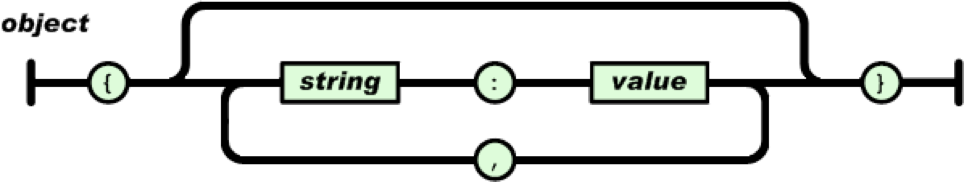
\includegraphics[width=0.8\textwidth]{figures/json-object}
\label{fig:json-object}
\caption{}
\end{figure}

\begin{figure}[H]
\centering
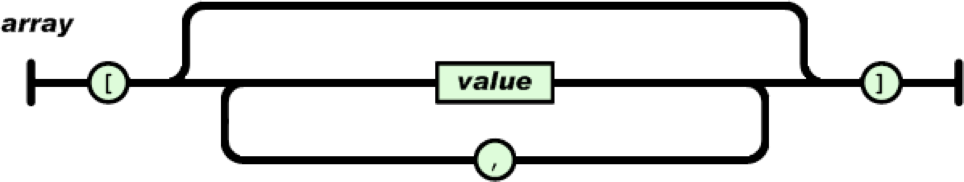
\includegraphics[width=0.8\textwidth]{figures/json-array}
\label{fig:json-array}
\caption{}
\end{figure}

\paragraph{} The values supported by JSON, together with the railroad mechanisms for constructing strings and numbers are given in the following diagrams.


\begin{figure}[H]
\centering
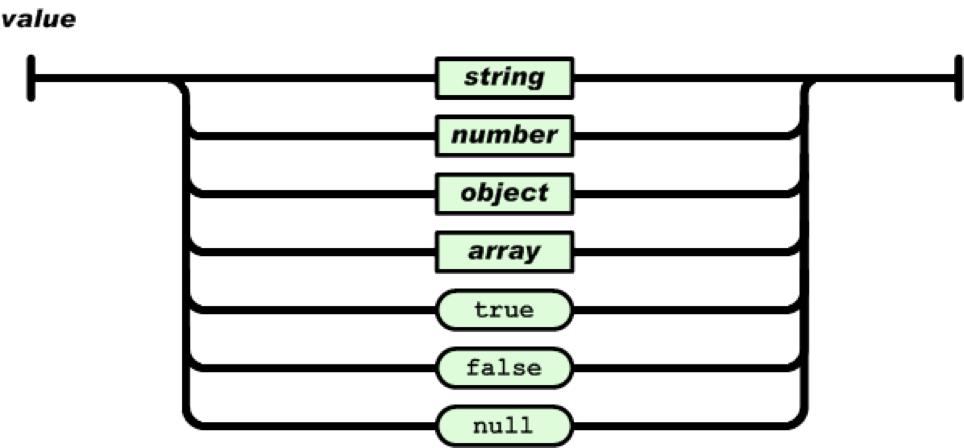
\includegraphics[width=0.8\textwidth]{figures/json-value}
\label{fig:json-value}
\caption{}
\end{figure}

\begin{figure}[H]
\centering
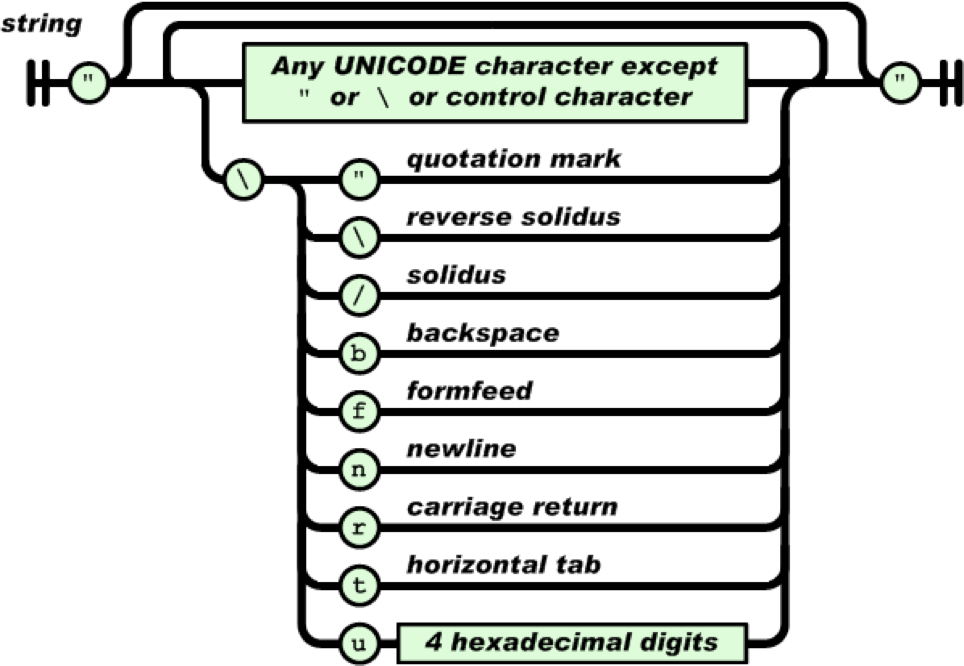
\includegraphics[width=0.8\textwidth]{figures/json-string}
\label{fig:json-string}
\caption{}
\end{figure}

\begin{figure}[H]
\centering
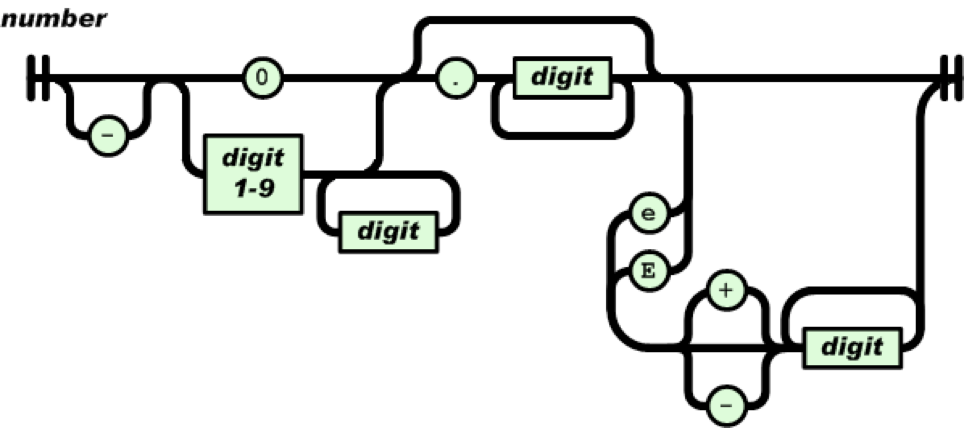
\includegraphics[width=0.8\textwidth]{figures/json-number}
\label{fig:json-number}
\caption{}
\end{figure}



\section{JSONLint}
\paragraph{} Linters are useful tools that are available for most programming languages. They are usually fairly simple programs that you can use to flag up programming errors. The kinds of errors that a Linter might bring to your attention can include syntax errors, certain kinds of bugs, stylistic issues, and various kinds of "code smell". Note that Linters can't (yet) check for more complicated or subtle bugs, for example, those arising from logical errors of reasoning that stem from the programmer, or from errors that arise because the problem and solution are underspecified, or because the programmer isn't sure what their goal is. Whenever you learn a new programming language it is worth looking for a linter tool to support you in using the language correctly and picking up on simple issues. Note that there is some overlap between a linter and the kinds of checks that some compilers and interpreters do but rather than going through the entire build process, which can be time consuming, a linter can process your source code and more rapidly give useful immediate feedback about certain categories of problems.
\paragraph{} JSONLint\footnote{\url{https://jsonlint.com/}} is a very useful online tool for quickly editing ad validating JSON files. You can find it here:	
\paragraph{} It's really simple to use, edit some JSON either in your own files then copy/pasting or directly into JSONLint's interface then press the "Validate JSON" button. The JSON is either valid or else you will be shown where the error lies. Once everything is fixed then you can copy and paste the nicely formatted JSON data back to your own text file and save for usage elsewhere.

\begin{figure}[H]
\centering
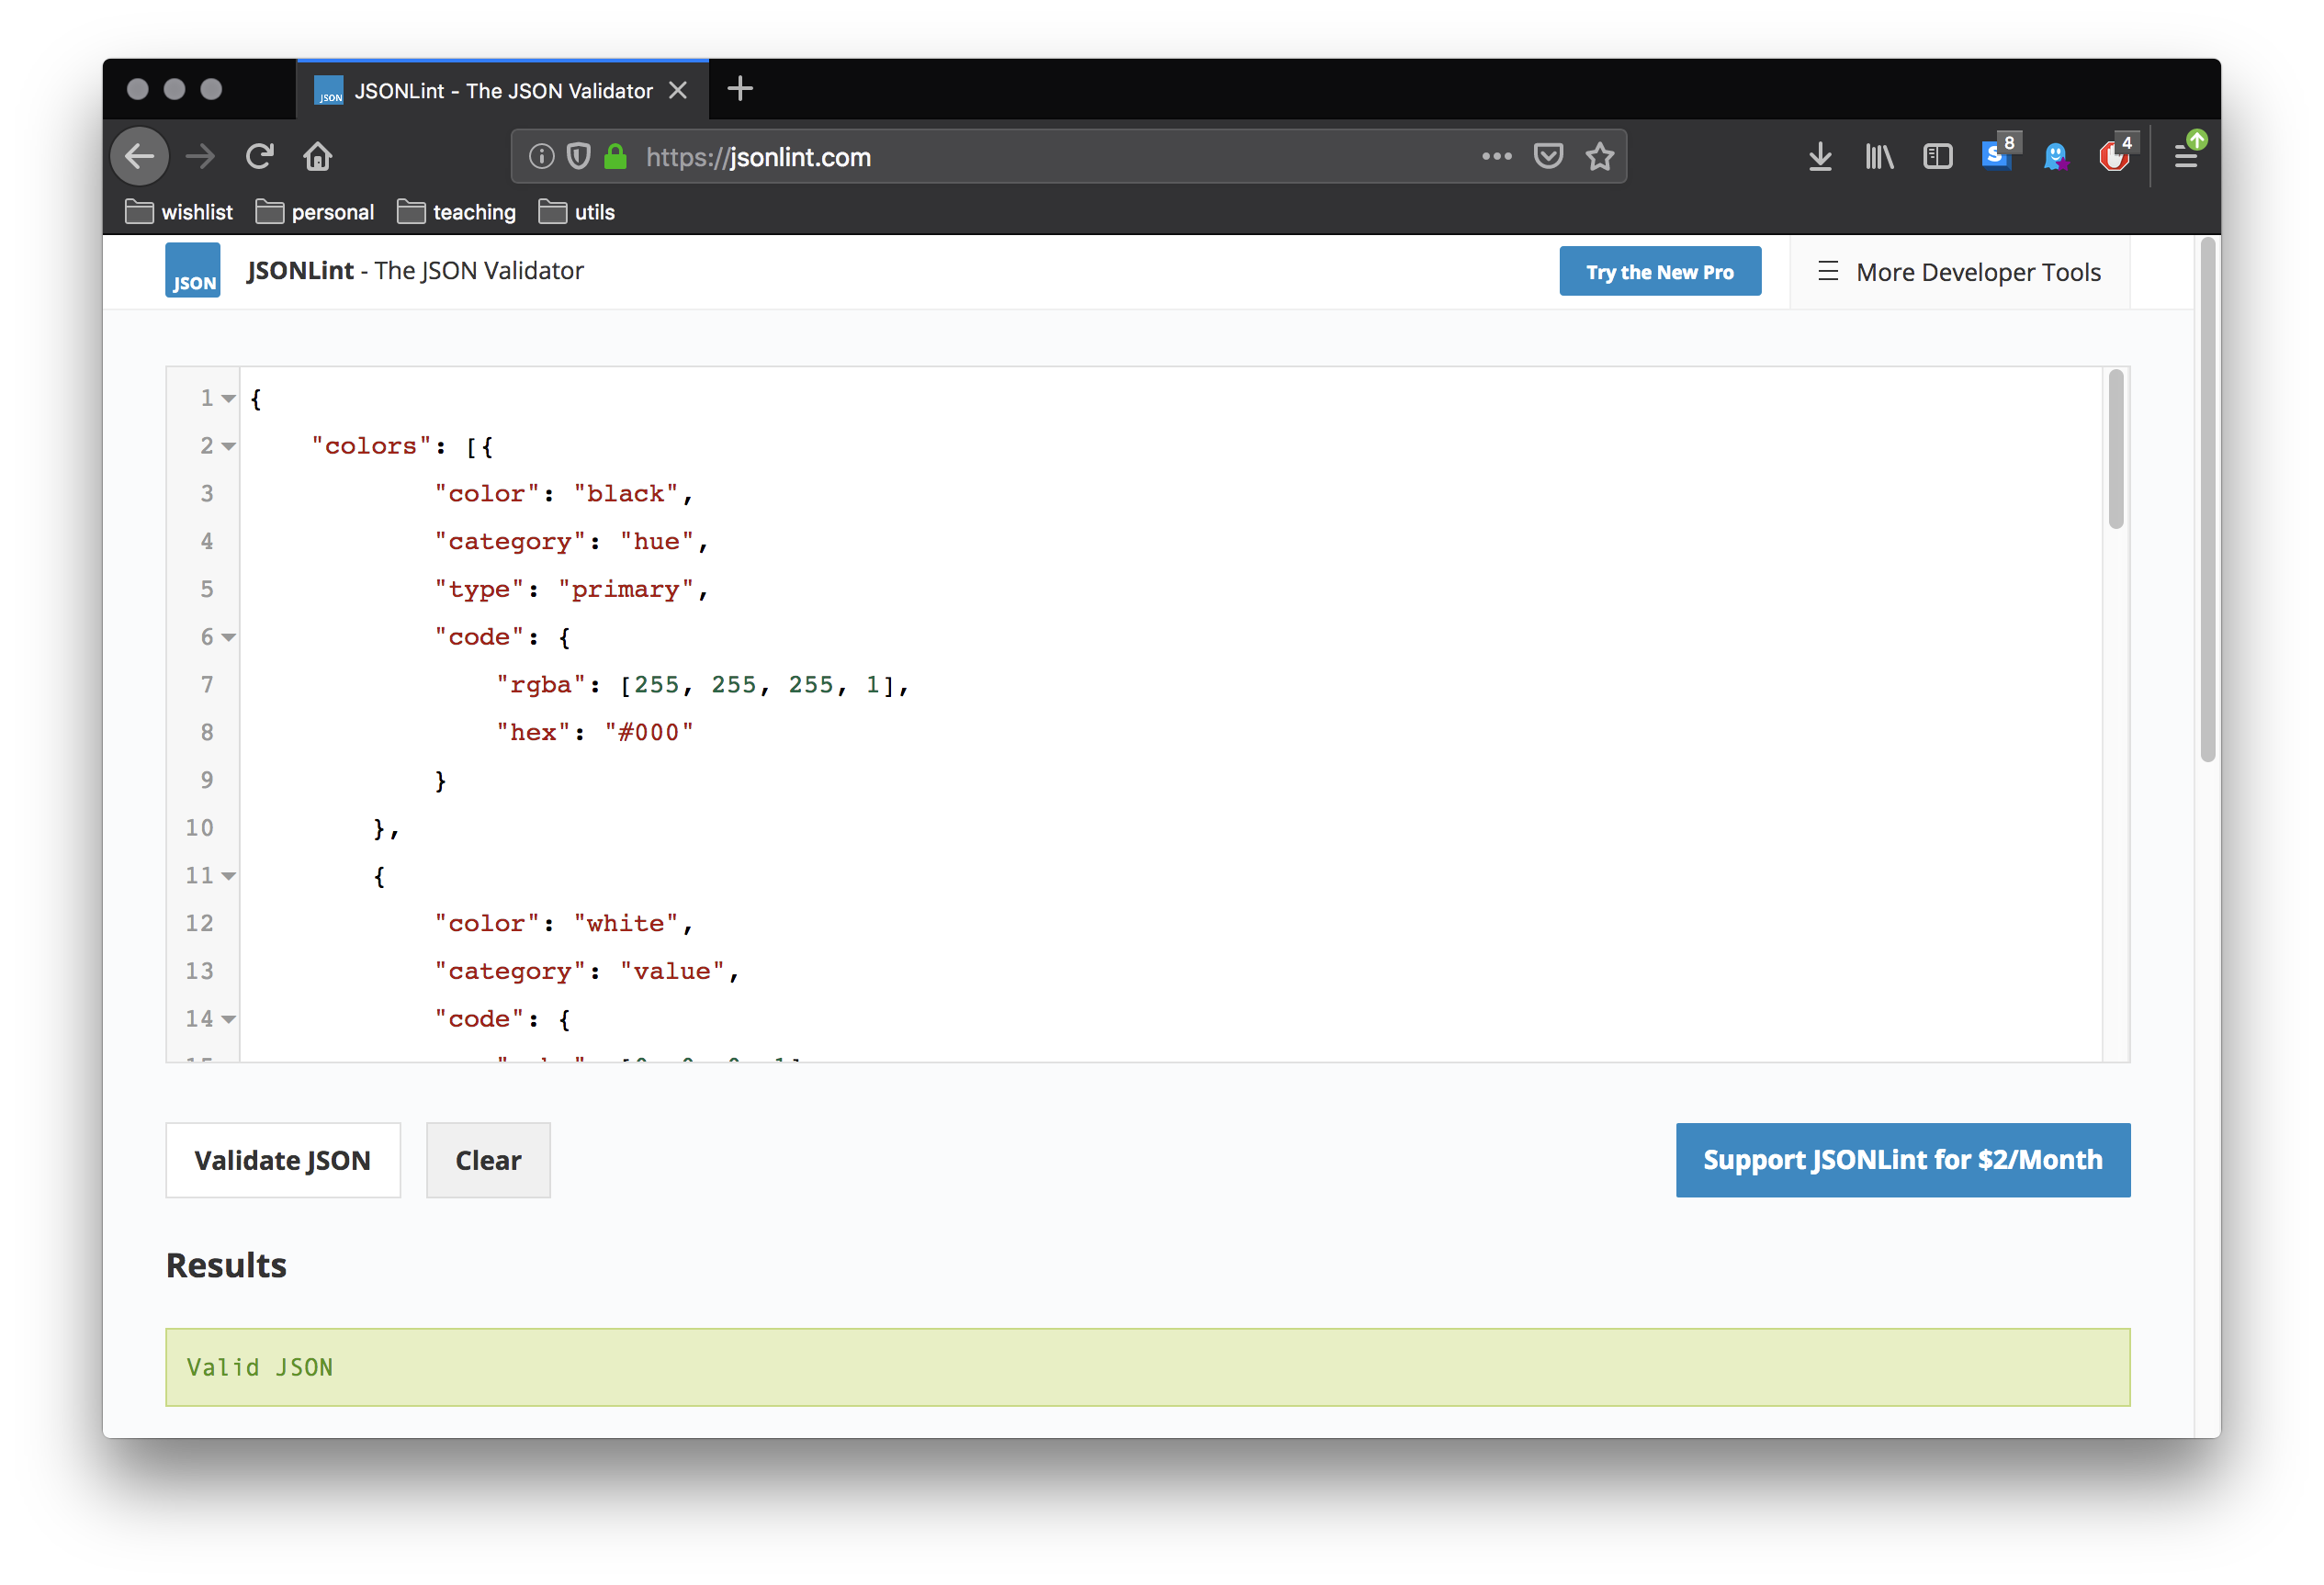
\includegraphics[width=0.8\textwidth]{figures/jsonlint}
\label{fig:jsonlint}
\caption{}
\end{figure}

\paragraph{} Note that JSONLint is also great for when you receive JSON from elsewhere, perhaps as the result of an API call. JSONLint will format the JSON and enable you to more easily see the structure of the data within the JSON document.


\section{Why is JSON important?}
\paragraph{} If you are going to build APIs, or really exploit JavaScript, or share data with other APIs (or retrieve data from them) then you will need to use JSON. Really, you can't effectively use JavaScript objects without getting a crash-course in JSON anyway, but JSON also has a role beyond being the text based serialisation format of JSON objects.
\paragraph{} There are many other data transport and representation languages, e.g. XML, YAML, RDF, but JSON occupies a sweet spot that:

\begin{itemize}
\item is not too complex — so you can get up and running swiftly and can quickly prototype ideas.
\item tooling is lightweight — you don't need any specialist tools, you can just write JSON into a regular text file (although as we saw earlier a Linter tool can be useful to help avoid simple mistakes).
\item is human readable — you should be able to read through a JSON document and interpret the structure of the data that it describes. If a JSON file isn't easily readable then that is usually either a failure of the developer of the file to ensure that it correctly communicates the data or else means that there is some specialist knowledge required to interpret the actual data itself, unrelated to the JSON representation.
\end{itemize}

\paragraph{} Yes, there are drawbacks to JSON (stackoverflow is a great place to find discussions between professional developers on the merits, or otherwise, of JSON), but the positives make it an easy tool to choose and use. This is probably why JSON is frequently a go to choice for data description and representation even amongst developers who are not doing web development or using JavaScript.

\section{Resources}
\paragraph{} As usual, due to the rapid pace of change in web technologies, the best place to get up to date information about the current status of browser related data storage APIs is from the Mozilla and Google documentation.

\begin{itemize}
\item MDN Cookie API\footnote{\url{https://developer.mozilla.org/en-US/docs/Web/API/Document/cookie}}
\item MDN Web Storage API\footnote{\url{https://developer.mozilla.org/en-US/docs/Web/API/Web_Storage_API}}
\item MDN Indexed DB API Documentation\footnote{\url{https://developer.mozilla.org/en-US/docs/Web/API/IndexedDB_API}}
\item Google Developers Documentation (Indexed DB)\footnote{\url{https://developers.google.com/web/ilt/pwa/working-with-indexeddb}}
\end{itemize}

\section{Summary}
\paragraph{} In this chapter we’ve looked at the following broad topics:
\begin{itemize}
\item Identified the current main approaches to data storage for the web
\item Distinguished between server-side and client-side data storage
\item Made appropriate choices about which technology to select for a given problem
\end{itemize}

